\documentclass[
12pt,
a4paper,
semrecuonosumario,
sumario = abnt-6027-2012]{report}

% --- Pacotes essenciais
\usepackage[T1]{fontenc}
\usepackage[utf8]{inputenc}
\usepackage[brazil]{babel}
\usepackage{geometry}
\geometry{a4paper,margin=2.5cm}
\usepackage{setspace}
\onehalfspacing
\usepackage{graphicx}
\usepackage{float}
\usepackage[hidelinks]{hyperref}
\usepackage{titlesec}
\usepackage{tocloft}
\usepackage{helvet}
\renewcommand{\familydefault}{\sfdefault}
\usepackage{ragged2e}
\usepackage{indentfirst}
\usepackage{subcaption}
\usepackage{amsmath}
\setcounter{MaxMatrixCols}{20}



% --- Listagens de código
\usepackage{listings}
\lstset{
	basicstyle=\ttfamily\small,
	breaklines=true,
	frame=single,
	numbers=left,
	numberstyle=\tiny,
	tabsize=2,
	literate={á}{{\'a}}1 {â}{{\^a}}1 {ã}{{\~a}}1 {à}{{\`a}}1
	{Á}{{\'A}}1 {Â}{{\^A}}1 {Ã}{{\~A}}1 {À}{{\`A}}1
	{é}{{\'e}}1 {ê}{{\^e}}1 {É}{{\'E}}1 {Ê}{{\^E}}1
	{í}{{\'i}}1 {Í}{{\'I}}1
	{ó}{{\'o}}1 {ô}{{\^o}}1 {õ}{{\~o}}1 {Ó}{{\'O}}1 {Ô}{{\^O}}1 {Õ}{{\~O}}1
	{ú}{{\'u}}1 {Ú}{{\'U}}1
	{ç}{{\c{c}}}1 {Ç}{{\c{C}}}1
}

% --- (Opcional) Lista de algoritmos – mantida para refletir o PDF
\usepackage{algorithm}
\usepackage{algpseudocode}

% --- Aparência dos títulos
% \titleformat{\chapter}{\bfseries}{\thechapter}{1em}{}
% \titleformat{\section}{\bfseries}{\thesection}{1em}{}
% \titleformat{\subsection}{\bfseries}{\thesubsection}{1em}{}

% --- Dados para a capa/rosto
\newcommand{\universidade}{UNIVERSIDADE TECNOLÓGICA FEDERAL DO PARANÁ}
\newcommand{\autores}{CAIO MACEDO\\ KAÍQUE MEDEIROS LIMA\\ IAN BATISTA FORNAZIERO}
\newcommand{\titulo}{MEMORIAL DESCRITIVO\\Algoritmos em Grafos}
\newcommand{\english}{Descriptive Memorial - Graph Algorithms}
\newcommand{\docente}{Dra. Leiliane Pereira de Rezende}
\newcommand{\cidade}{SANTA HELENA}
\newcommand{\periodo}{2025/2}

\begin{document}
	
	% --- Capa
	\begin{titlepage}
		\centering
		{\bf \universidade\par}
		\vspace{4cm}
		{\bf\autores\par}
		\vspace{6cm}
		{\bf\titulo\par}
		\vspace{9cm}
		{\bf\cidade\par}
		{\bf\periodo\par}
		\newpage
		
		{\bf\autores\par}
		\vspace{3.5cm}
		{\bf\titulo\par}
		\vspace{2cm}
		{\bf\english\par}
		\vspace{3cm}
		\begin{flushright} % alinha o bloco à direita
			\begin{minipage}{0.5\textwidth} % ocupa metade da largura do texto
				\justifying % vem do pacote ragged2e
				\noindent
				Trabalho de Conclusão de Disciplina de
				Graduação apresentado como requisito para
				conclusão da disciplina de Algoritmos em
				Grafos do Curso de Bacharelado em Ciência
				da Computação da Universidade Tecnológica
				Federal do Paraná
				
				\vspace{1em}
				\noindent
				Docente: Dra. Leiliane Pereira de Rezende
			\end{minipage}
		\end{flushright}
		\vspace{5cm}
		{\bf\cidade\par}
		{\bf\periodo\par}
		\thispagestyle{empty}
	\end{titlepage}
	\newpage
	\setcounter{page}{1}
	\section*{\centering \small\bfseries LISTA DE ALGORITMOS}
	
	\newpage
	\section*{\centering \small\bfseries LISTA DE FIGURAS}
	
	\newpage
	\section*{\centering \small\bfseries LISTAGEM DE CÓDIGOS FONTE}
	
	\newpage
	\section*{\centering \small\bfseries LISTA DE ABREVIATURAS E SIGLAS}
	\textbf{Siglas}\\
	
	\noindent
	ACID\hspace{1cm}Atomicidade, Consistência, Isolamento e Durabilidade
	\clearpage
	
	\renewcommand{\cftdotsep}{1}
	
	% --- Título do sumário (compatível com tocloft antigo)
	\renewcommand{\contentsname}{\MakeUppercase{Sumário}}
	\renewcommand{\cfttoctitlefont}{\bfseries\small} % estilo e tamanho
	\renewcommand{\cftaftertoctitle}{\hfill\par}           % segundo \hfill centraliza
	\renewcommand{\cftchapfont}{\bfseries}
	\renewcommand{\cftchappagefont}{\bfseries}
	
	% --- seções normais (sem negrito)
	\renewcommand{\cftsecfont}{\bfseries}
	\renewcommand{\cftsecpagefont}{\bfseries}
	
	% --- subseções também normais
	\renewcommand{\cftsubsecfont}{\bfseries}
	\renewcommand{\cftsubsecpagefont}{\bfseries}
	
	\setlength{\cftbeforetoctitleskip}{0pt}
	\setlength{\cftaftertoctitleskip}{2ex}
	
	% Larguras/recuos (alinham número/título/página)
	\cftsetindents{chapter}{1em}{4.0em}
	\cftsetindents{section}{1em}{4.0em}
	\cftsetindents{subsection}{0em}{0em}
	
	% Profundidade do sumário (0=chap, 1=sec, 2=subsec, ...)
	\setcounter{tocdepth}{2}
	\tableofcontents
	\newpage
	
	\titleformat{\chapter}{\bfseries\small}{\thechapter}{1em}{}
	\titlespacing*{\chapter}{0pt}{2.5ex}{1.5ex}
	\titleformat{\section}{\bfseries\small}{\thesection}{1em}{}
	\titlespacing*{\section}{0pt}{2.0ex}{1.0ex}
	
	
	\chapter{INTRODUÇÃO} \label{cap:introducao}
	
	A estrutura de dados grafos é aplicada em diversas áreas do conhecimento, as quais podem ser esquematizadas via um conjunto de conexões entre pares de objetos. A descrição do problema a ser trabalhado em todo o documento é dada na Seção \ref{sec:descGrafo}. A composição do restante do documento é descrita na Seção \ref{sec:estruturaTrabalho}.
	
	\section{Descrição do Problema}\label{sec:descGrafo}
	O problema a ser modelado diz respeito a logística de transporte de uma
	empresa qualquer, que utiliza veículos automotivos como caminhões e carros. Esse meio de transporte tem como caracteristica a alta emissão de gases de efeito estufa (GEEs), que colaboram a degradação do meio ambiente. Nesse
	contexto, para amenizar o problema, deseja-se encontrar a melhor rota de um
	ponto a outro de forma sustentável. Por exemplo, se a empresa deseja realizar
	uma entrega de um ponto de distribuição a outro, a escolha da rota modelada por
	meio dos grafos levará em a emissão de GEEs do veículo, de acordo com o combustível utilizado e o consumo por quilometro. A melhor rota
	será aquela que possui o mínimo de emissão possível. Dessa forma, os impactos ao meio ambiente são minimizados,
	evitando a intensificação do aquecimento global. É importante destacar que, o caminho com menos emissão de GEEs pode também ser a rota mais econômica. A equação que define a emissão de GEEs por Litro é dada por:
	\begin{equation}
		 EF_{CO2,L}=\rho\ \times fc\ \times OF\ \times\frac{44}{12} 
	\end{equation}
	\\
	Onde,
	\begin{itemize}
		\item O $\rho$ é  a densidade do combustível
		\item o $fc$ é a fração mássica de carbono no combustível ($kgC/kg combustível$)
		\item OF é o fator de oxidação ($\approx 0.99 - 10$; a fração do carbono efetivamente oxidada a $CO_2$)
		\item $\frac{44}{12}$  converte $C \rightarrow CO_2$ (massa molar). 
	\end{itemize}
	A emissão total é dada pela multiplicação de emissão por litro e os litros.

	\section{Estrutura do Trabalho}\label{sec:estruturaTrabalho}
	A estrutura de dados grafo pode ser representada por diferentes meios, seja ela na visão computacional ou não. O capítulo \ref{cap:representacoes} apresenta tanto as representações não computacionais quanto as computacionais mais usadas nos algoritmos em grafos.
	
	No contexto da estrutura de dados grafo, diversas são as terminologias e tipagens existentes e, na sua grande maioria, independentes se o grafo é ou não orientado. No Capítulo \ref{cap:definicoesGrafo}, as principais terminologias e tipos que o grafo apresentado no Capítulo \ref{cap:introducao} contempla são descritos.
	
	Para facilitar ou solucionar alguns problemas modelados por meio da estrutura de grafos,  algumas operações matemática nos seus conjuntos de vértices e arestas são necessárias. As principais operações são exemplificadas no Capítulo \ref{cap:operacoes}.
	
	A busca é umas das técnicas mais aplicadas na solução de problemas algorítmicos em grafos considerados eficientes. O Capítulo \ref{cap:buscas} apresenta tanto a busca em largura quanto a busca em profundidade, bem como uma aplicação das duas para obter os componentes fortemente conexos de um grafo.
	
	Dentre as subestruturas de grafo que oferecem solução para problemas aplicados, os caminhos se destacam especialmente pelo potencial associado aos problemas de trânsito, transporte, localização em sistemas discretos, dentre outros. Quando a definição de distância é associada aos caminhos, surgem os problemas de caminho mínimo. O Capítulo \ref{cap:caminhoMinimo} apresenta o cálculo do caminho mínimo tanto para grafos não valorados quanto para valorados.
	
	Problemas de interligação (comunicações, redes de luz, água, esgotos, etc.) podem ser solucionados pela obtenção da árvore de cobertura de peso mínimo quando existe o interesse em se proceder à interligação de todos os pontos atendidos com o consumo mínimo de meios. O Capítulo \ref{cap:arvCobMinima} apresenta os dois algoritmos mais conhecidos na literatura para a obtenção de uma árvore de cobertura de peso mínimo.
	
	A modelagem e solução de um problema de ciclos por Leonard Euler, durante o século XVIII, é responsável por definir os fundamentos da teoria dos grafos. O teorema definido por Euler demostra se é possível ou não, a partir de algum ponto do grafo, percorrer todas as arestas uma única vez e voltar ao ponto de partida. No Capítulo \ref{cap:grafosEulerianos}, o grafo apresentado geometricamente na Figura \ref{fig:grafGeometrico} é verificado se satisfaz ou não o teorema de Euler. Caso, sim, o grafo é dito Euleriano. Caso contrário, uma eulerização é aplicada para obter um ciclo com o menor número de arestas/arcos repetidos.
	
	Problemas de roteamento como comunicação, logística, e, com ligeiras modificações, perfuração de placas de circuito impresso, entre outros, têm com a mesma premissa: a partir de algum ponto, percorrer todos os outros uma única vez e voltar ao ponto de partida. Semelhante ao problema de grafos eulerianos, este problema, nomeado de ciclo hamiltoniano, não conhece uma condição necessária e suficiente que seja trivial para verificar a existência ou não deste ciclo. O Capítulo \ref{cap:grafosHamiltonianos} aplica o teorema mais importante, o teorema de Dirac, o teorema de Ore que é usado para deduzí-lo, além do teorema de Bondy e Chvátal no grafo estudado. Adicionalmente, mostra a (in)existência de um ciclo hamiltoniano também no grafo estudado.
	
	O Capítulo \ref{cap:emparelhamento} apresenta as principais definições do problema de emparelhamento. Este problema pode ser aplicado em problemas de atribuição de pessoal, de casamentos, de construção de amostras, entre outros. A ideia geral é formar o maior conjunto de pares de vértices adjacentes somente entre si.
	
	A planaridade de um projeto é questão importante em diversas situações práticas, como circuitos, cartografia, malhas de transporte terrestre e aéreo, construção de viadutos, entre outros. O Capítulo \ref{cap:planaridade} verifica a planaridade do grafo estudado.
	
	Problemas de competição/conflito por algum recurso, como a resolução de quebra-cabeças de Sudoku, podem ser solucionados pelo problema de coloração de grafos. O Capítulo \ref{cap:coloracaoVertices} apresenta a aplicação de um algoritmo guloso para uma solução e, por meio do conceito das cadeias de Kempe, verifica se existe outra solução com um número cromático menor.
	
	
	\chapter{Representações de um Grafo}\label{cap:representacoes}
	
	Um grafo pode ser representado por diferentes meios, seja ele na visão computacional ou não. Considerando a visão não computacional, o grafo pode ser representado tanto matematicamente quanto geometricamente. O primeiro modo é descrito na Seção \ref{sec:matematica} e o segundo na Seção \ref{sec:geometrica}, ambos considerando a descrição do grafo dado no Capítulo \ref{cap:introducao}.
	
	A representação por meio da visão computacional pode ser dada por três meios: matriz de adjacência, lista de adjacência e matriz de incidência. A descrição de cada um destes meios é dada, respectivamente, nas Seções \ref{sec:matriz}, \ref{sec:lista}, e \ref{sec:incidencia}. As considerações acerca da eficiência computacional, tanto em relação ao tempo de processamento quanto ao espaço usado de memória, são dadas na Seção \ref{sec:eficienciaRepresentacao}.
	
	
	\section{Matemática}\label{sec:matematica}
	
	A representação matemática do nosso problema é:\\ 
	$ G_1 = {\{V_1,A_1\}} $\\
	$V_1 = {\{1,2,3,4,5,6,7,8,9,10,11,12,13,14,15, 16}\}$\\
	$A_1 = {\{a_1,a_2,a_3,a_4,a_5,a_6,a_7,a_8,a_9,a_{10}, a_{11},a_{12},a_{13},a_{14},a_{15},a_{16}, a_{17}, a_{18}, a_{19}, a_{20}, a_{21}, a_{22}\}}$\\
	onde, \\
	$a_1 = (1,2) $; $a_2 = (1,3) $; $a_3 = (1,4) $; $a_4 = (2,6) $; $a_5 = (3,11) $; $a_6 = (4,7) $; $a_7 = (4,5) $; $a_8 = (5,8) $;
	$a_9 = (6,9) $; $a_{10} = (6,10) $; $a_{11} = (10,11) $; $a_{12} = (7,11) $; $a_{13} = (7,12) $; $a_{14} = (8,12) $; $a_{15} = (11,12) $; $a_{16} = (9,13) $;
	$a_{17} = (13,10) $; $a_{18} = (11,15) $; $a_{19} = (12,15) $; $a_{20} = (13,14) $; $a_{21} = (14,15) $; $a_{22} = (15,16) $.\\
	Cada vértice representa uma localidade na região da cidade de santa helena sendo elas:
	\begin{itemize}
		\item 1: Santa Helena
		\item 2: Entre Rios do Oeste
		\item 3: Diamante D'oeste
		\item 4: Missal
		\item 5: Itaipulândia
		\item 6: São José das Palmeiras
		\item 7: Ramilândia
		\item 8: Medianeira
		\item 9: Ouro Verde do Oeste 
		\item 10: São Pedro do Iguaçu
		\item 11: Vera Cruz do Oeste
		\item 12: Matelândia
		\item 13: Toledo
		\item 14: Cascavel
		\item 15: Santa Tereza do Oeste
		\item 16:Lindoeste
	\end{itemize}
	
	\section{Geométrica}\label{sec:geometrica}
	\begin{figure}[!htb]%% Ambiente figure
	\caption{Representação Geométrica do Grafo}%% Legenda
		\label{fig:grafGeometrico}%% Rótulo
		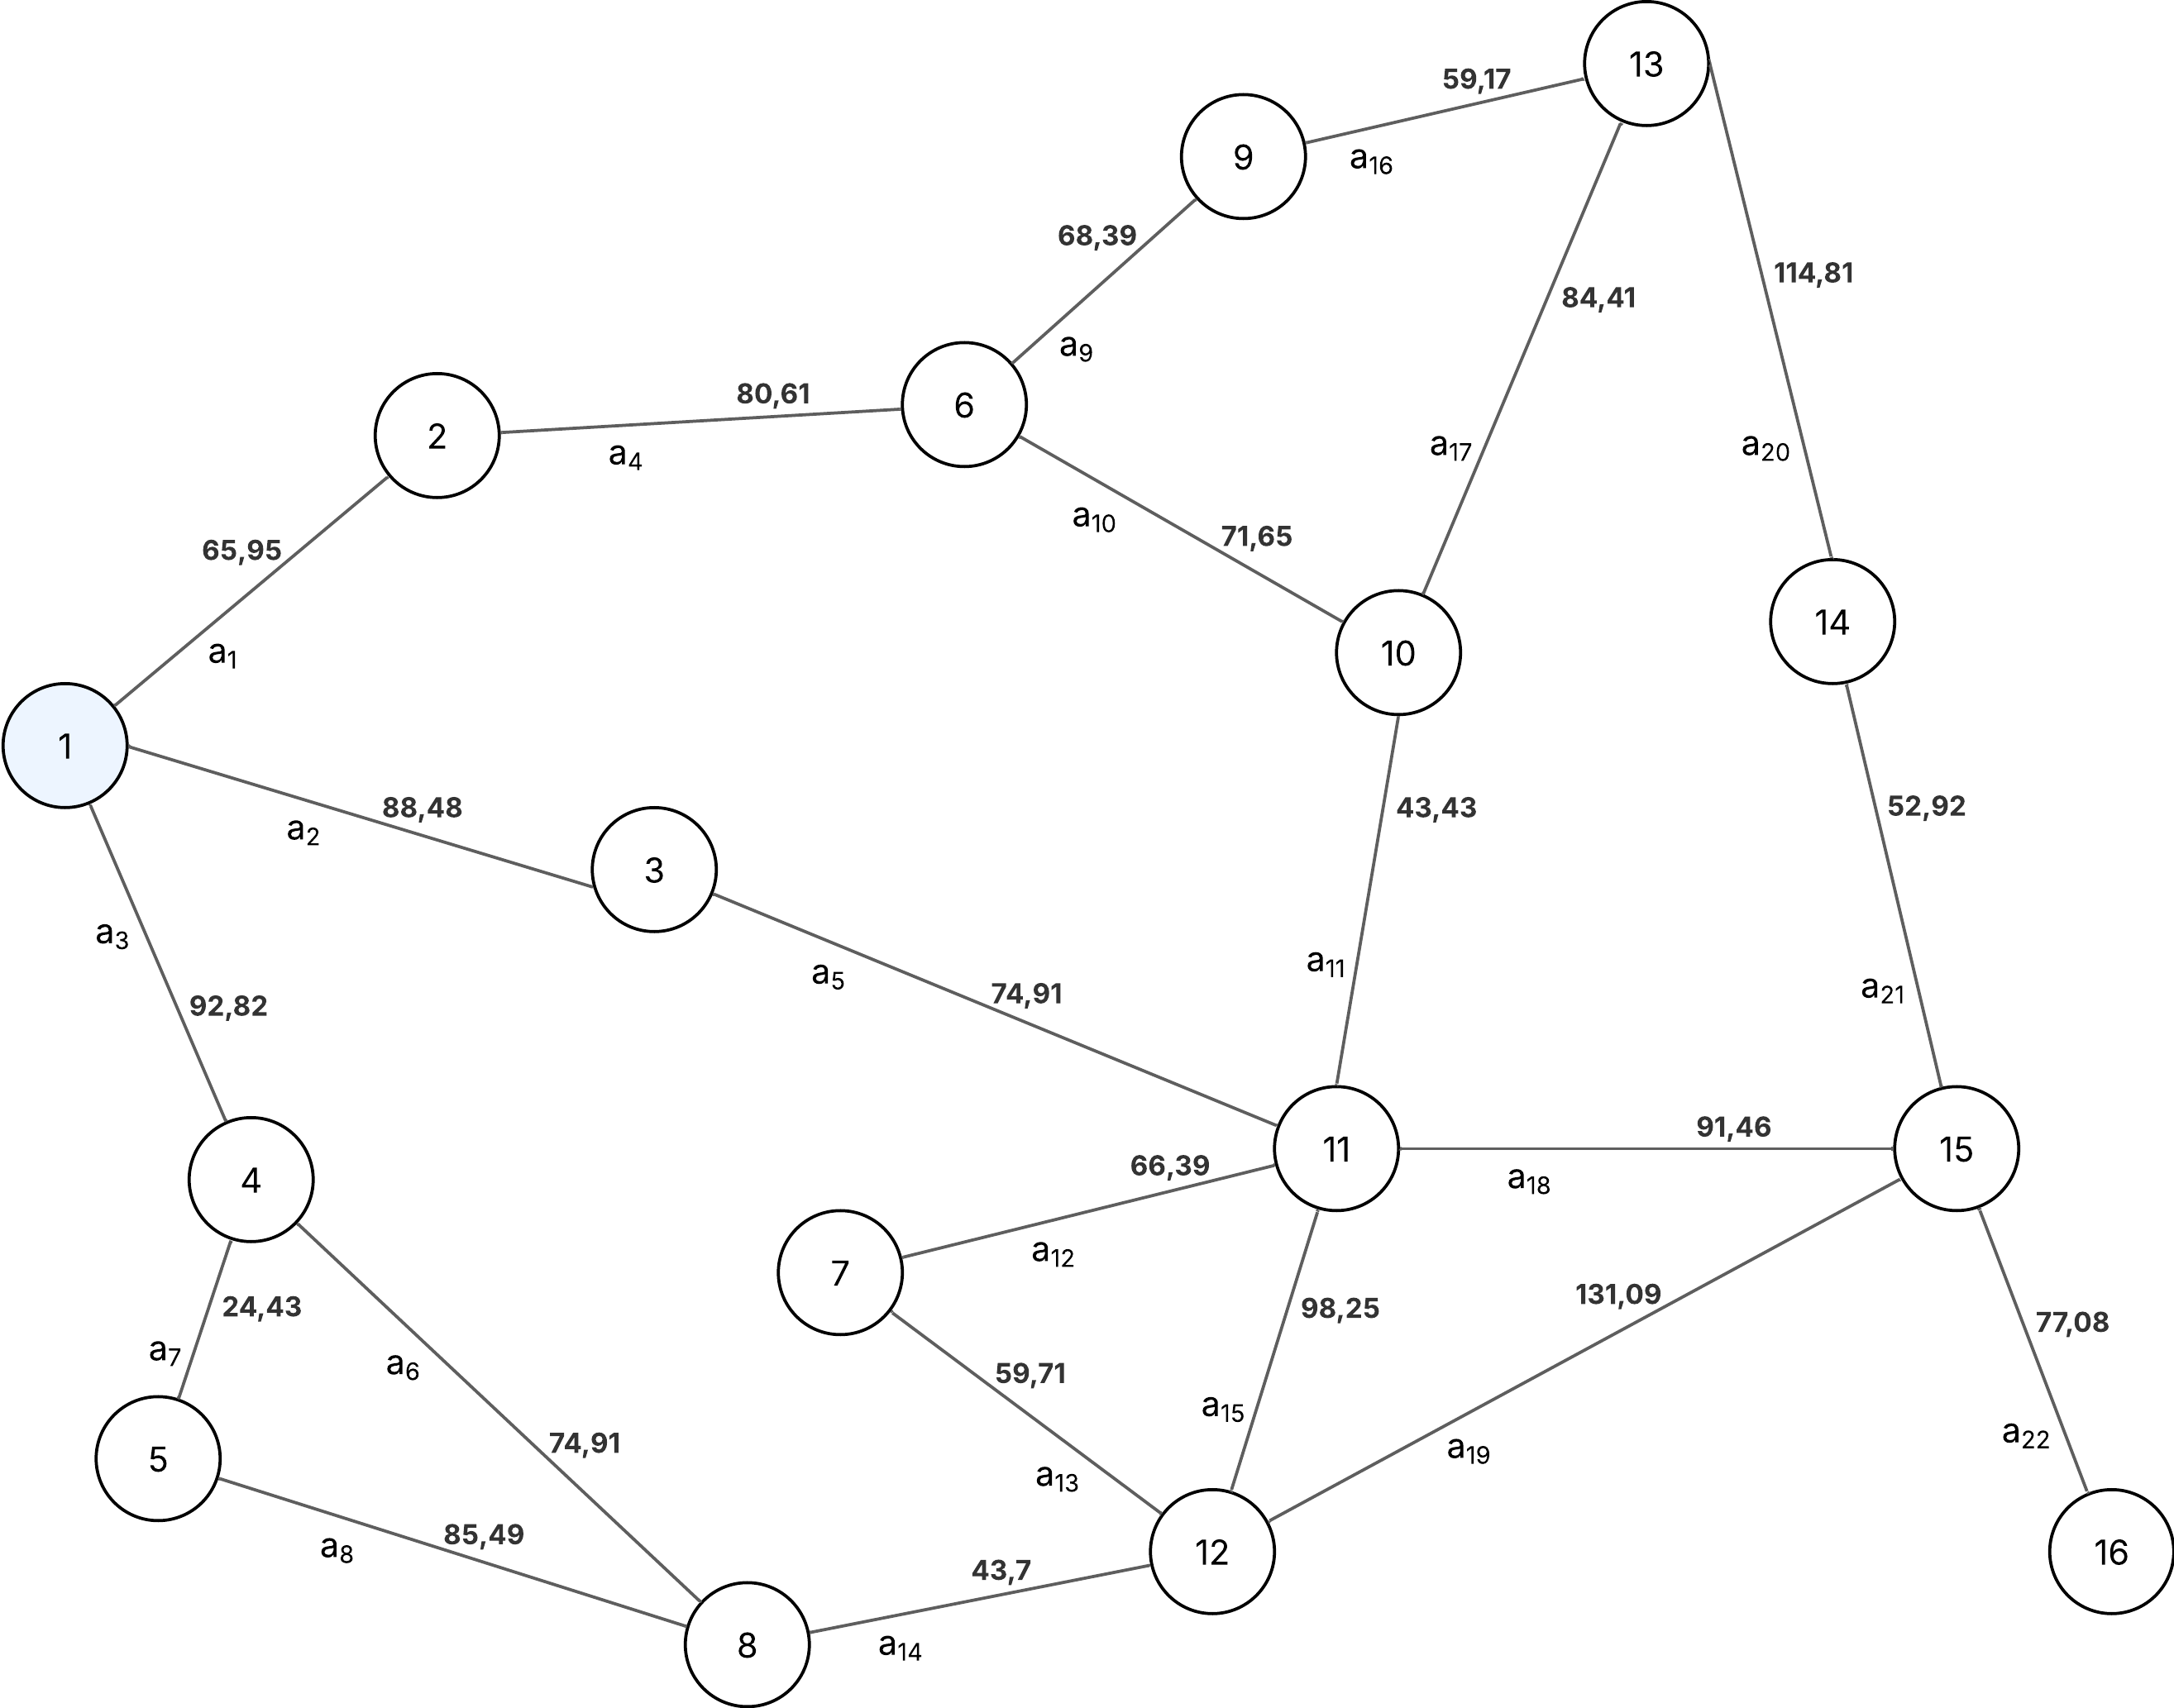
\includegraphics[width=1\textwidth,angle=0]{figuras/grafoGeometrico.png}%% Dimensões e localização
	\centering{Fonte: Criação própria}%% Fonte
	\end{figure}
	
	
	\section{Matriz de Adjacência}\label{sec:matriz}
	
	A matriz de Adjacência do nosso problema é:
	

	\[
	\begin{bmatrix}
		0 & 1 & 1 & 1 & 0 & 0 & 0 & 0 & 0 & 0 & 0 & 0 & 0 & 0 & 0 & 0\\% 1
		1 & 0 & 0 & 0 & 0 & 1 & 0 & 0 & 0 & 0 & 0 & 0 & 0 & 0 & 0 & 0\\% 2
		1 & 0 & 0 & 0 & 0 & 0 & 0 & 0 & 0 & 0 & 1 & 0 & 0 & 0 & 0 & 0\\% 3
		1 & 0 & 0 & 0 & 1 & 0 & 0 & 1 & 0 & 0 & 0 & 0 & 0 & 0 & 0 & 0\\% 4
		0 & 0 & 0 & 1 & 0 & 0 & 0 & 1 & 0 & 0 & 0 & 0 & 0 & 0 & 0 & 0\\% 5
		0 & 1 & 0 & 0 & 0 & 0 & 0 & 0 & 1 & 1 & 0 & 0 & 0 & 0 & 0 & 0\\% 6
		0 & 0 & 0 & 0 & 0 & 0 & 0 & 0 & 0 & 0 & 1 & 1 & 0 & 0 & 0 & 0\\% 7
		0 & 0 & 0 & 1 & 1 & 0 & 0 & 0 & 0 & 0 & 0 & 1 & 0 & 0 & 0 & 0\\% 8 
		0 & 0 & 0 & 0 & 0 & 1 & 0 & 0 & 0 & 0 & 0 & 0 & 1 & 0 & 0 & 0\\% 9 
		0 & 0 & 0 & 0 & 0 & 1 & 0 & 0 & 0 & 0 & 1 & 0 & 1 & 0 & 0 & 0\\% 10
		0 & 0 & 1 & 0 & 0 & 0 & 1 & 0 & 0 & 1 & 0 & 1 & 0 & 0 & 1 & 0\\% 11
		0 & 0 & 0 & 0 & 0 & 0 & 1 & 1 & 0 & 0 & 1 & 0 & 0 & 0 & 1 & 0\\% 12
		0 & 0 & 0 & 0 & 0 & 0 & 0 & 0 & 1 & 1 & 0 & 0 & 0 & 1 & 0 & 0\\% 13 
		0 & 0 & 0 & 0 & 0 & 0 & 0 & 0 & 0 & 0 & 0 & 0 & 1 & 0 & 1 & 0\\% 14
		0 & 0 & 0 & 0 & 0 & 0 & 0 & 0 & 0 & 0 & 1 & 1 & 0 & 1 & 0 & 1\\% 15
		0 & 0 & 0 & 0 & 0 & 0 & 0 & 0 & 0 & 0 & 0 & 0 & 0 & 0 & 1 & 0 % 16
	\end{bmatrix}
	\]

	
	\section{Lista de Adjacência}\label{sec:lista}
	
	A lista de Adjacência do nosso problema é:
	
	\section{Matriz de Incidência}\label{sec:incidencia}
	
	A matriz de Incidência do nosso problema é:
	
	\section{Considerações de Eficiência}\label{sec:eficienciaRepresentacao}
	
	\chapter{Definições em um Grafo }\label{cap:definicoesGrafo}

	Como a estrutura de dados grafo é uma estrutura heterogenia, definições são necessárias para compreender partes ou o todo da estrutura. Na Seção \ref{sec:terminologias}, as principais terminologias, considerando o grafo representado graficamente na Figura  \ref{fig:grafGeometrioco}, são apresentadas. Enquanto, na Seção \ref{sec:tiposGrafos}, todos os tipos os quais o grafo estudado contempla são apresentados.

	\section{Terminologias}\label{sec:terminologias}


	\section{Tipos de Grafos}\label{sec:tiposGrafos}

		
	\chapter{Operações}\label{cap:operacoes}
	
	A estrutura de dados grafos permitem algumas operações matemáticas nos seus conjuntos de vértices e arestas de modo a facilitar a execução de alguns algoritmos. As principais operações são: união, intersecção, soma, decomposição, remoção, fusão e contração. Cada uma delas são exemplificadas, respectivamente, nas Seções \ref{sec:uniao}, \ref{sec:interseccao}, \ref{sec:soma}, \ref{sec:decomposicao}, \ref{sec:remocao}, \ref{sec:fusao} e \ref{sec:contracao}.
	
	\section{União}\label{sec:uniao}
        A união de dois grafos, sendo eles $G_1 = (V_1, A_1)$ e $G_2 = (V_2, A_2)$, é dada por:
        \[
        G_1 \cup G_2 = (V_1 \cup V_2, A_1 \cup A_2)
        \]

        Esta é uma operação que apenas une os vértices e arestas dos grafos envolvidos, não adicionando nenhuma outra parte.
        Temos como exemplo a adição do $Sub\_Grafo1$ ao grafo $Sub\_Grafo2$.
        Onde $Sub\_Grafo1 = (V_1, V_2, V_3, V_6, V_{10}, V_{11}, a_1, a_2, a_4, a_5, a_{10}, a_{11} )$ e $Sub\_Grafo2 = (V_6, V_9, V_{10}, V_{11}, V_{13}, V_{14}, V_{15}, A_{9}, A_{10}, A_{11}, A_{16}, A_{17}, A_{18}, A_{20}, A_{21})$.

        % TEMPLATE ADICIONAR IMAGEM EM LATEX
        % \begin{figure}[!h]
        %     \centering
        % 	\label{fig:uniaoGrafos}
        % 	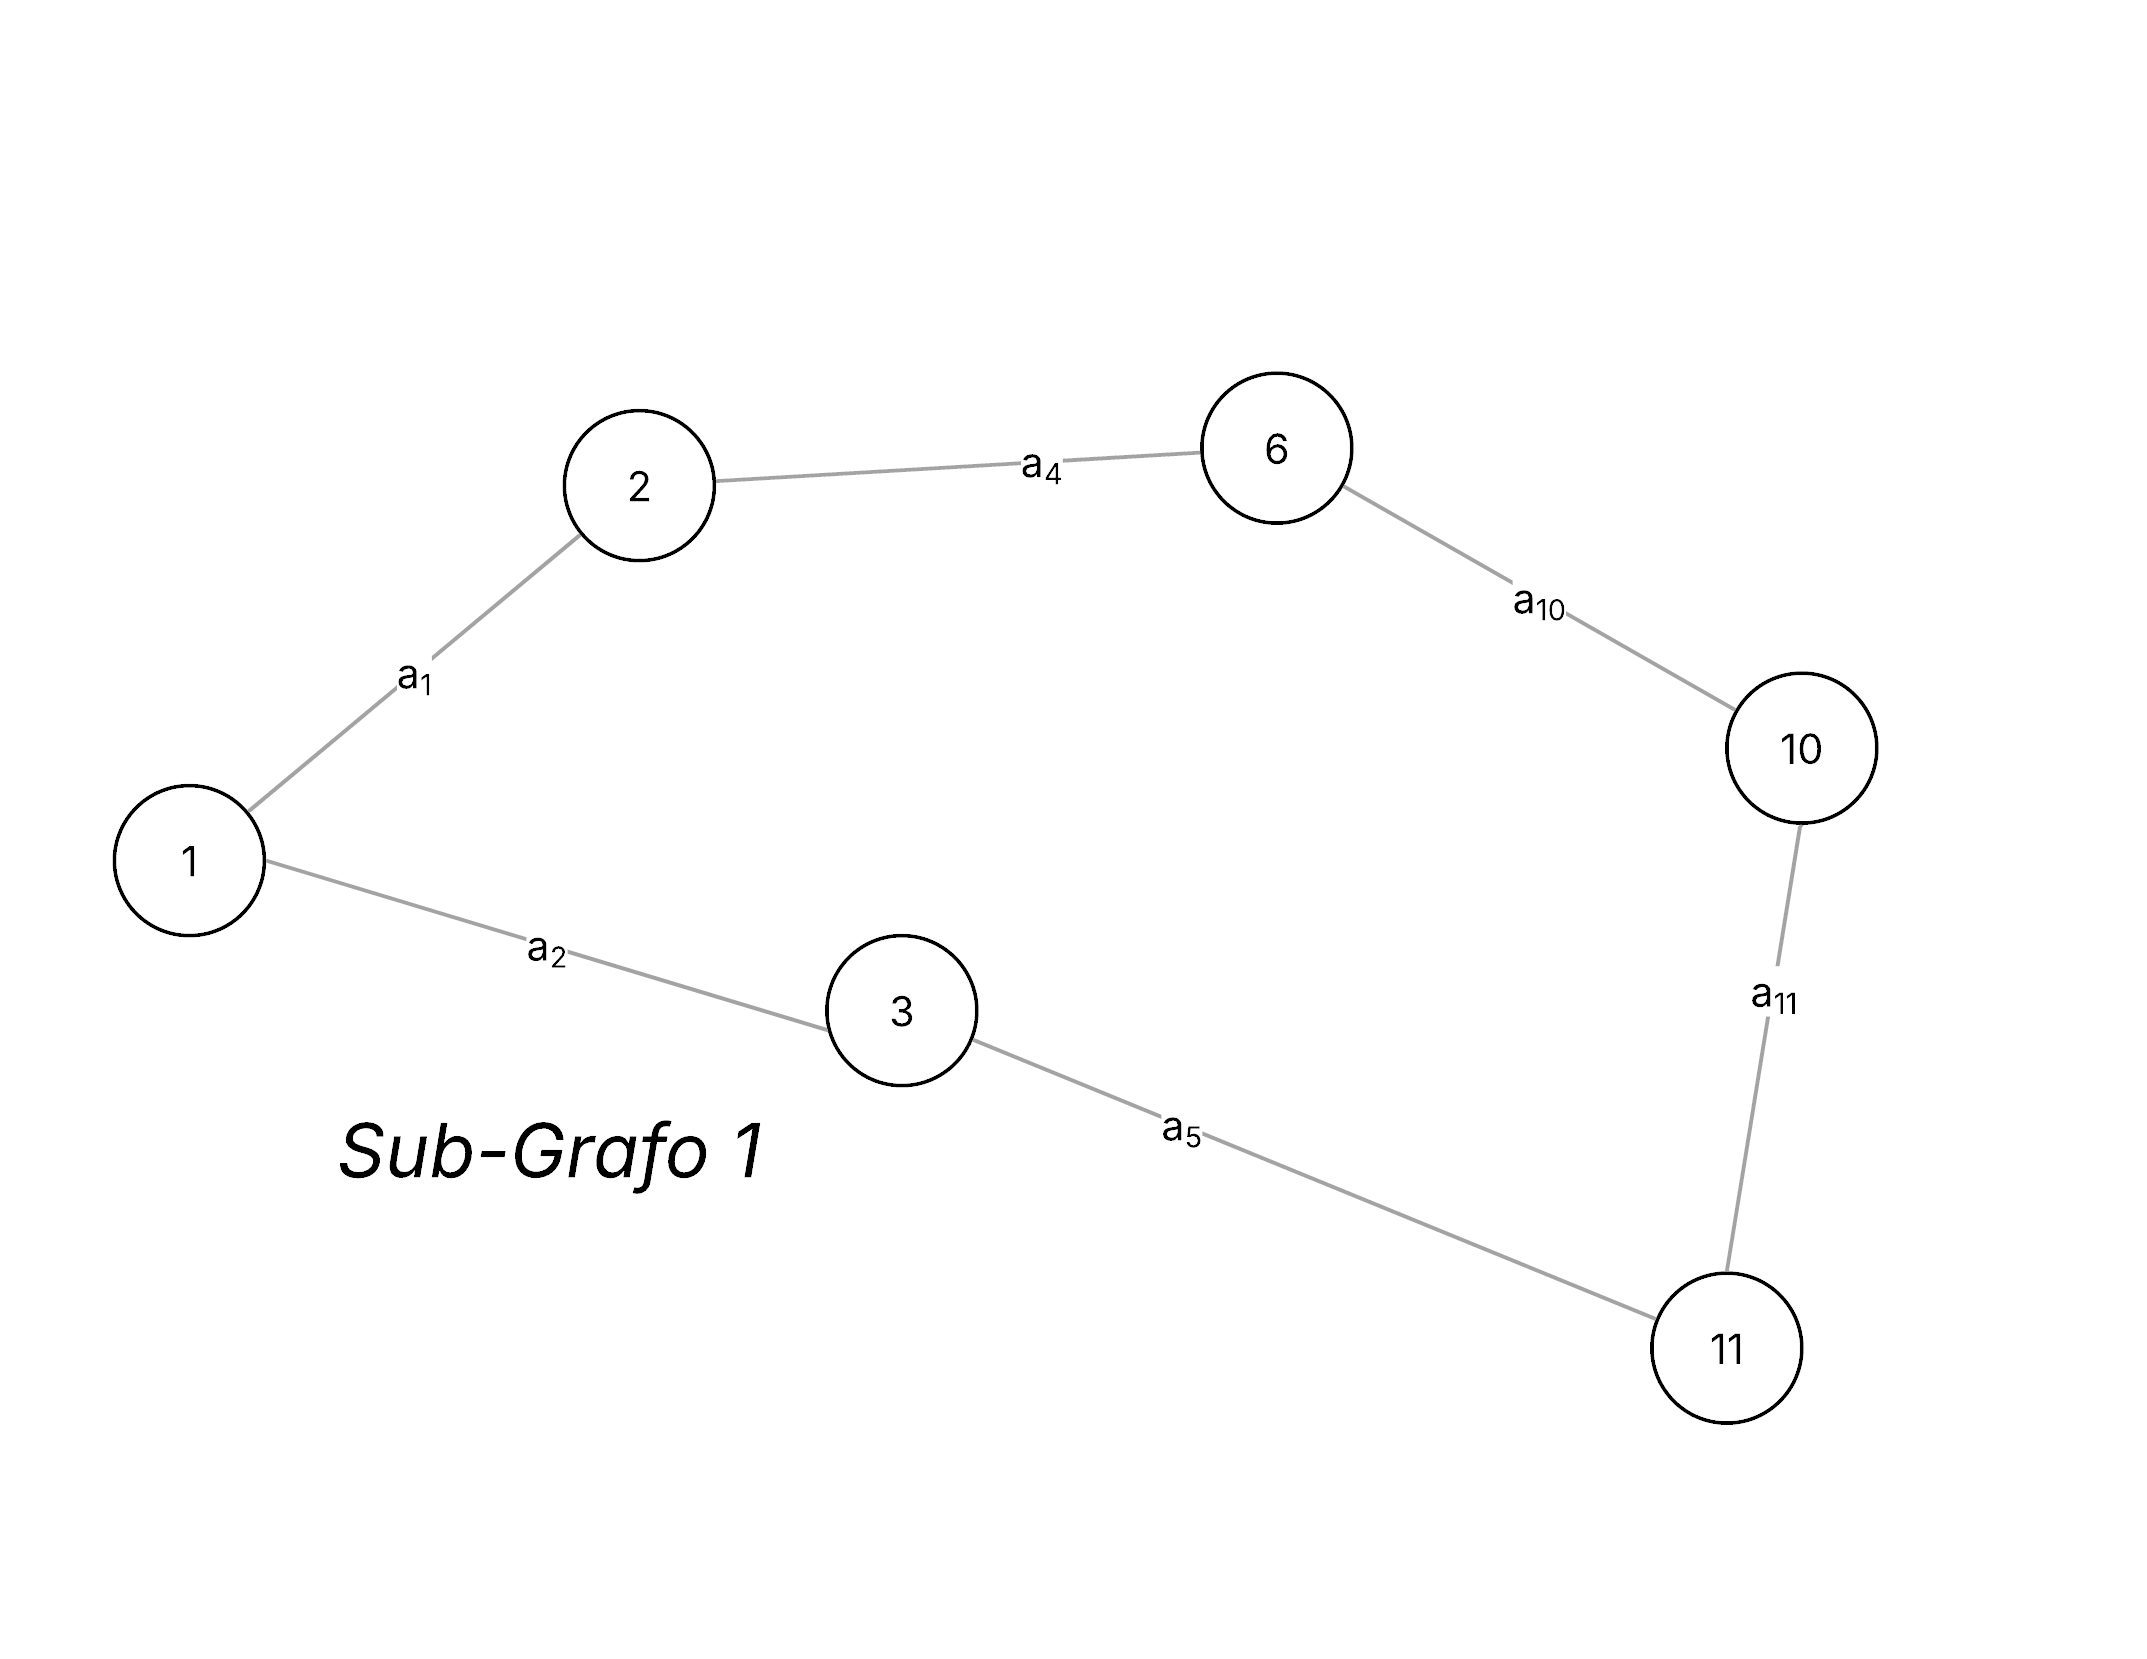
\includegraphics[width=0.7\textwidth]{figuras/subgrafos/subgrafo1.png}
        % 	\caption{Sub-Grafo 1}
        % \end{figure}
        \begin{figure}[!htb]
            \centering % Centraliza o conjunto de subfiguras na página

            \begin{subfigure}[b]{0.48\textwidth}
                \centering
                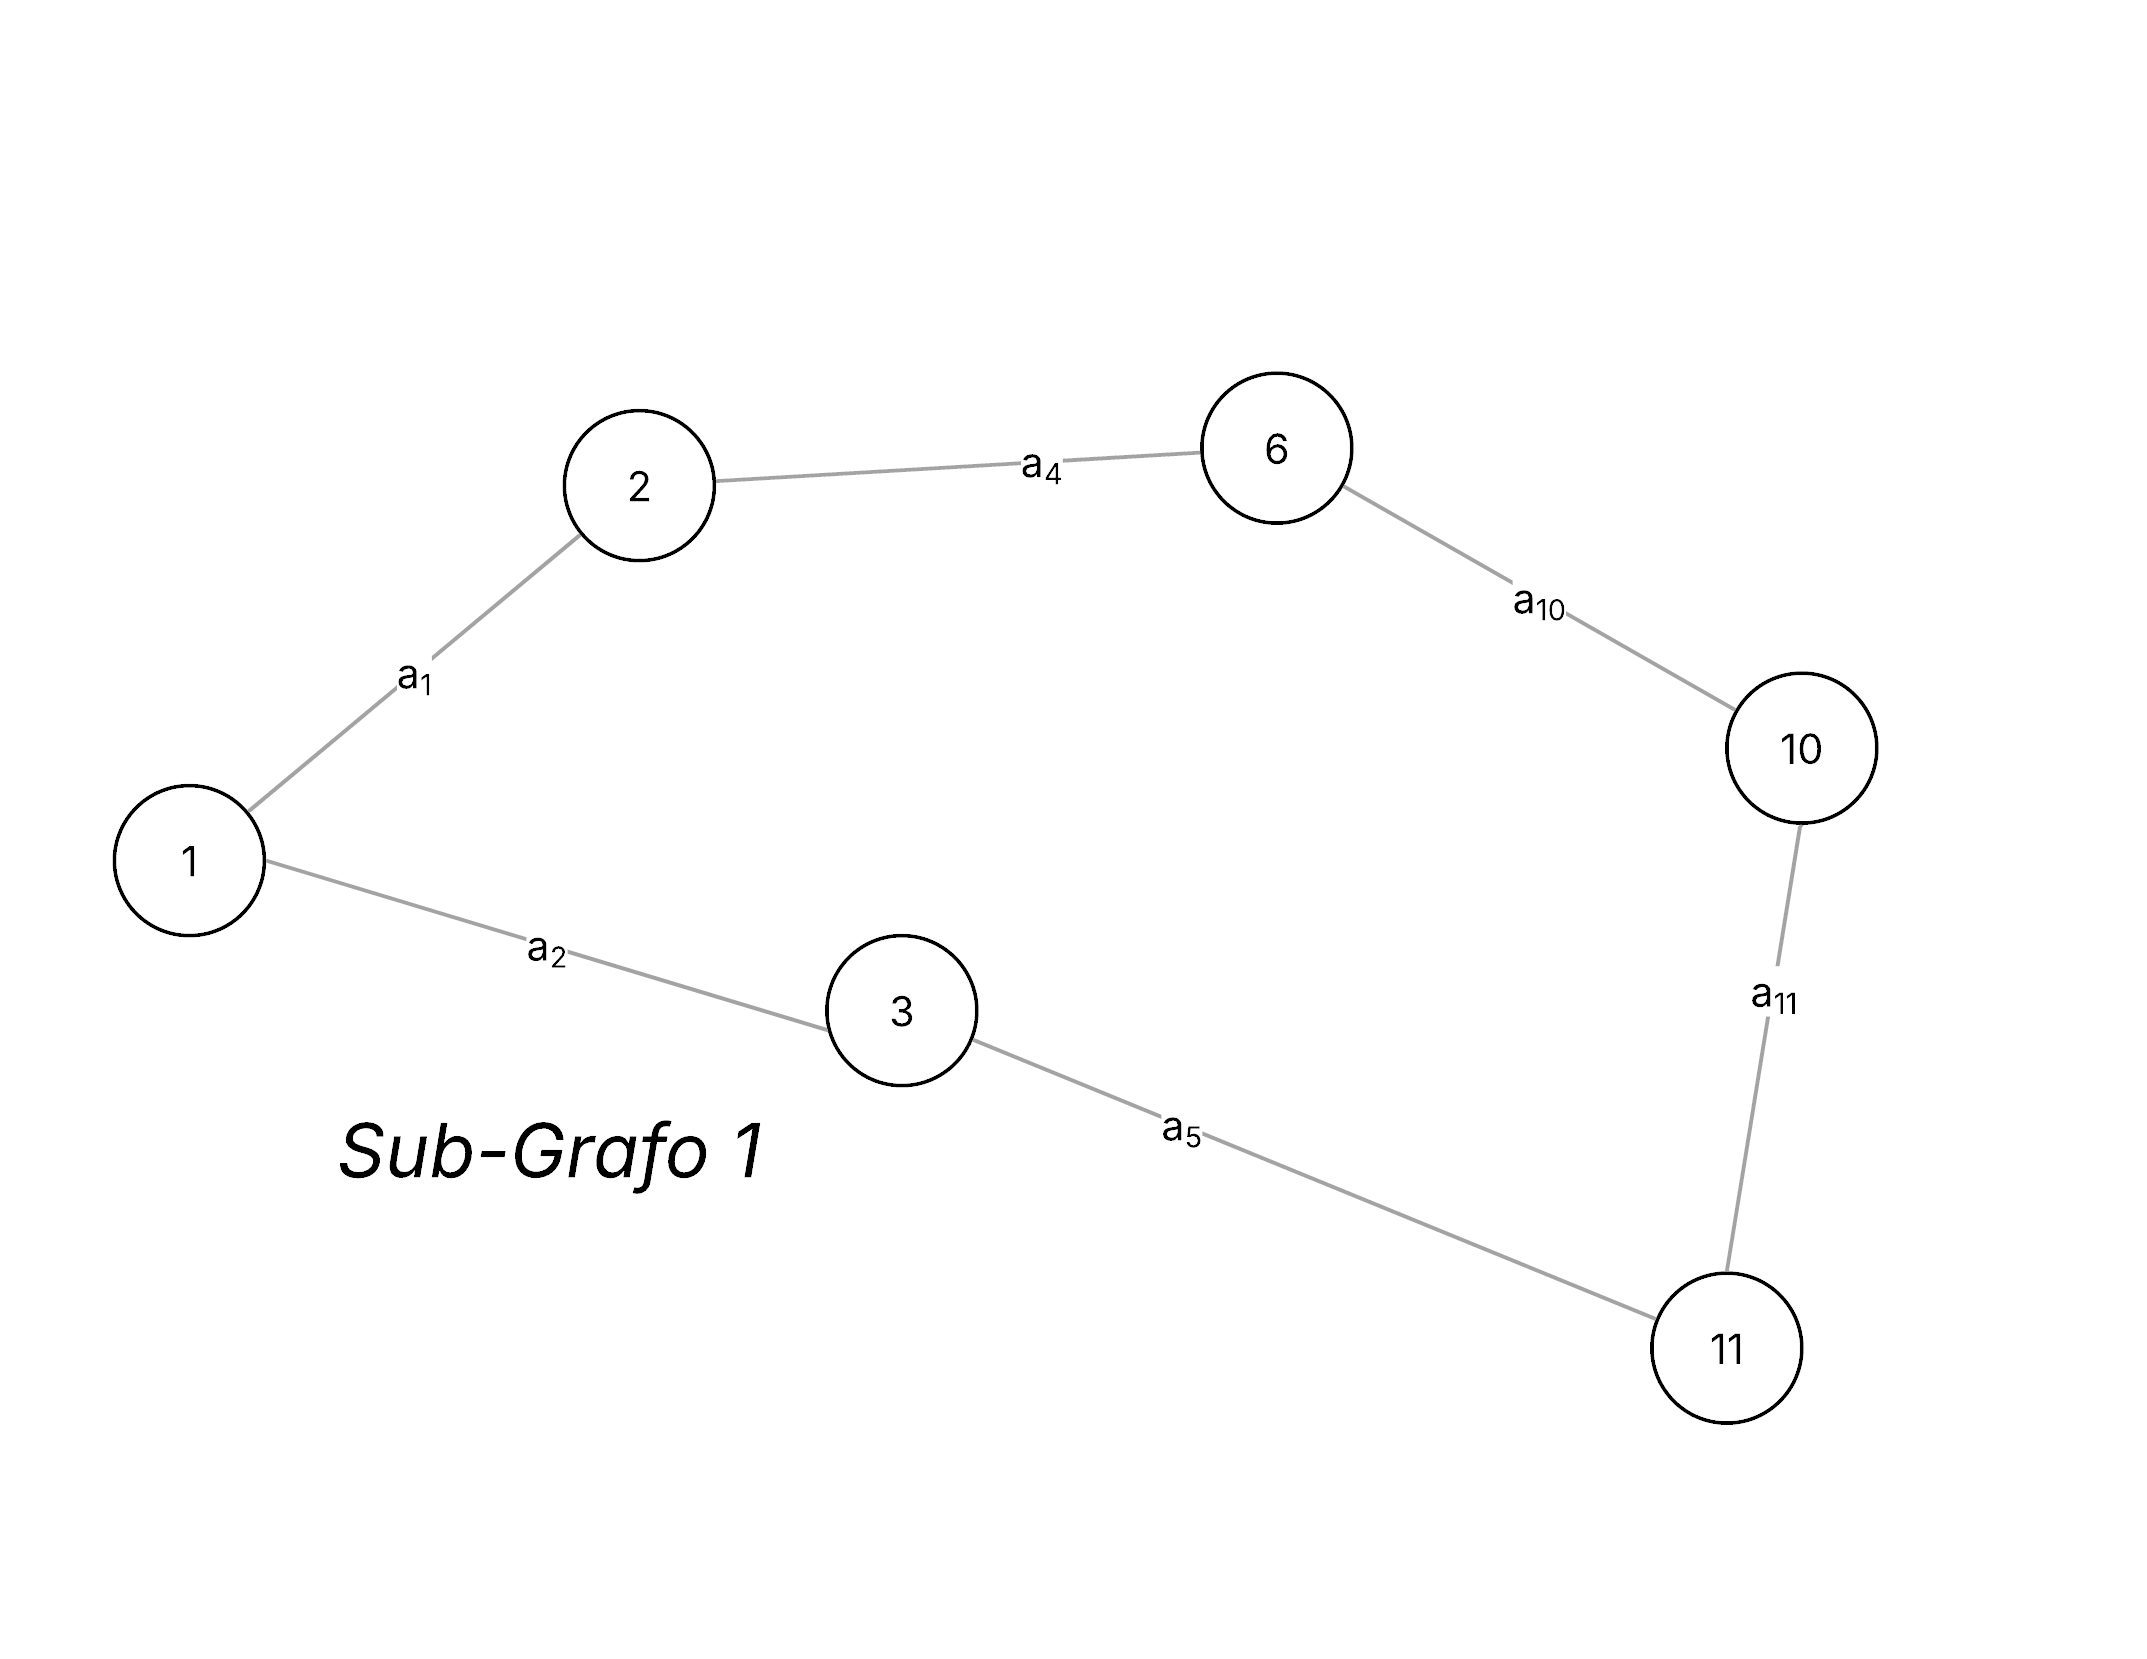
\includegraphics[width=\textwidth]{figuras/subgrafos/subgrafo1.png} % Substitua pelo caminho da sua imagem
                \caption{Sub-Grafo 1}
                \label{fig:imagem1}
            \end{subfigure}
            \hfill % Adiciona um espaço flexível entre as imagens
            \begin{subfigure}[b]{0.48\textwidth}
                \centering
                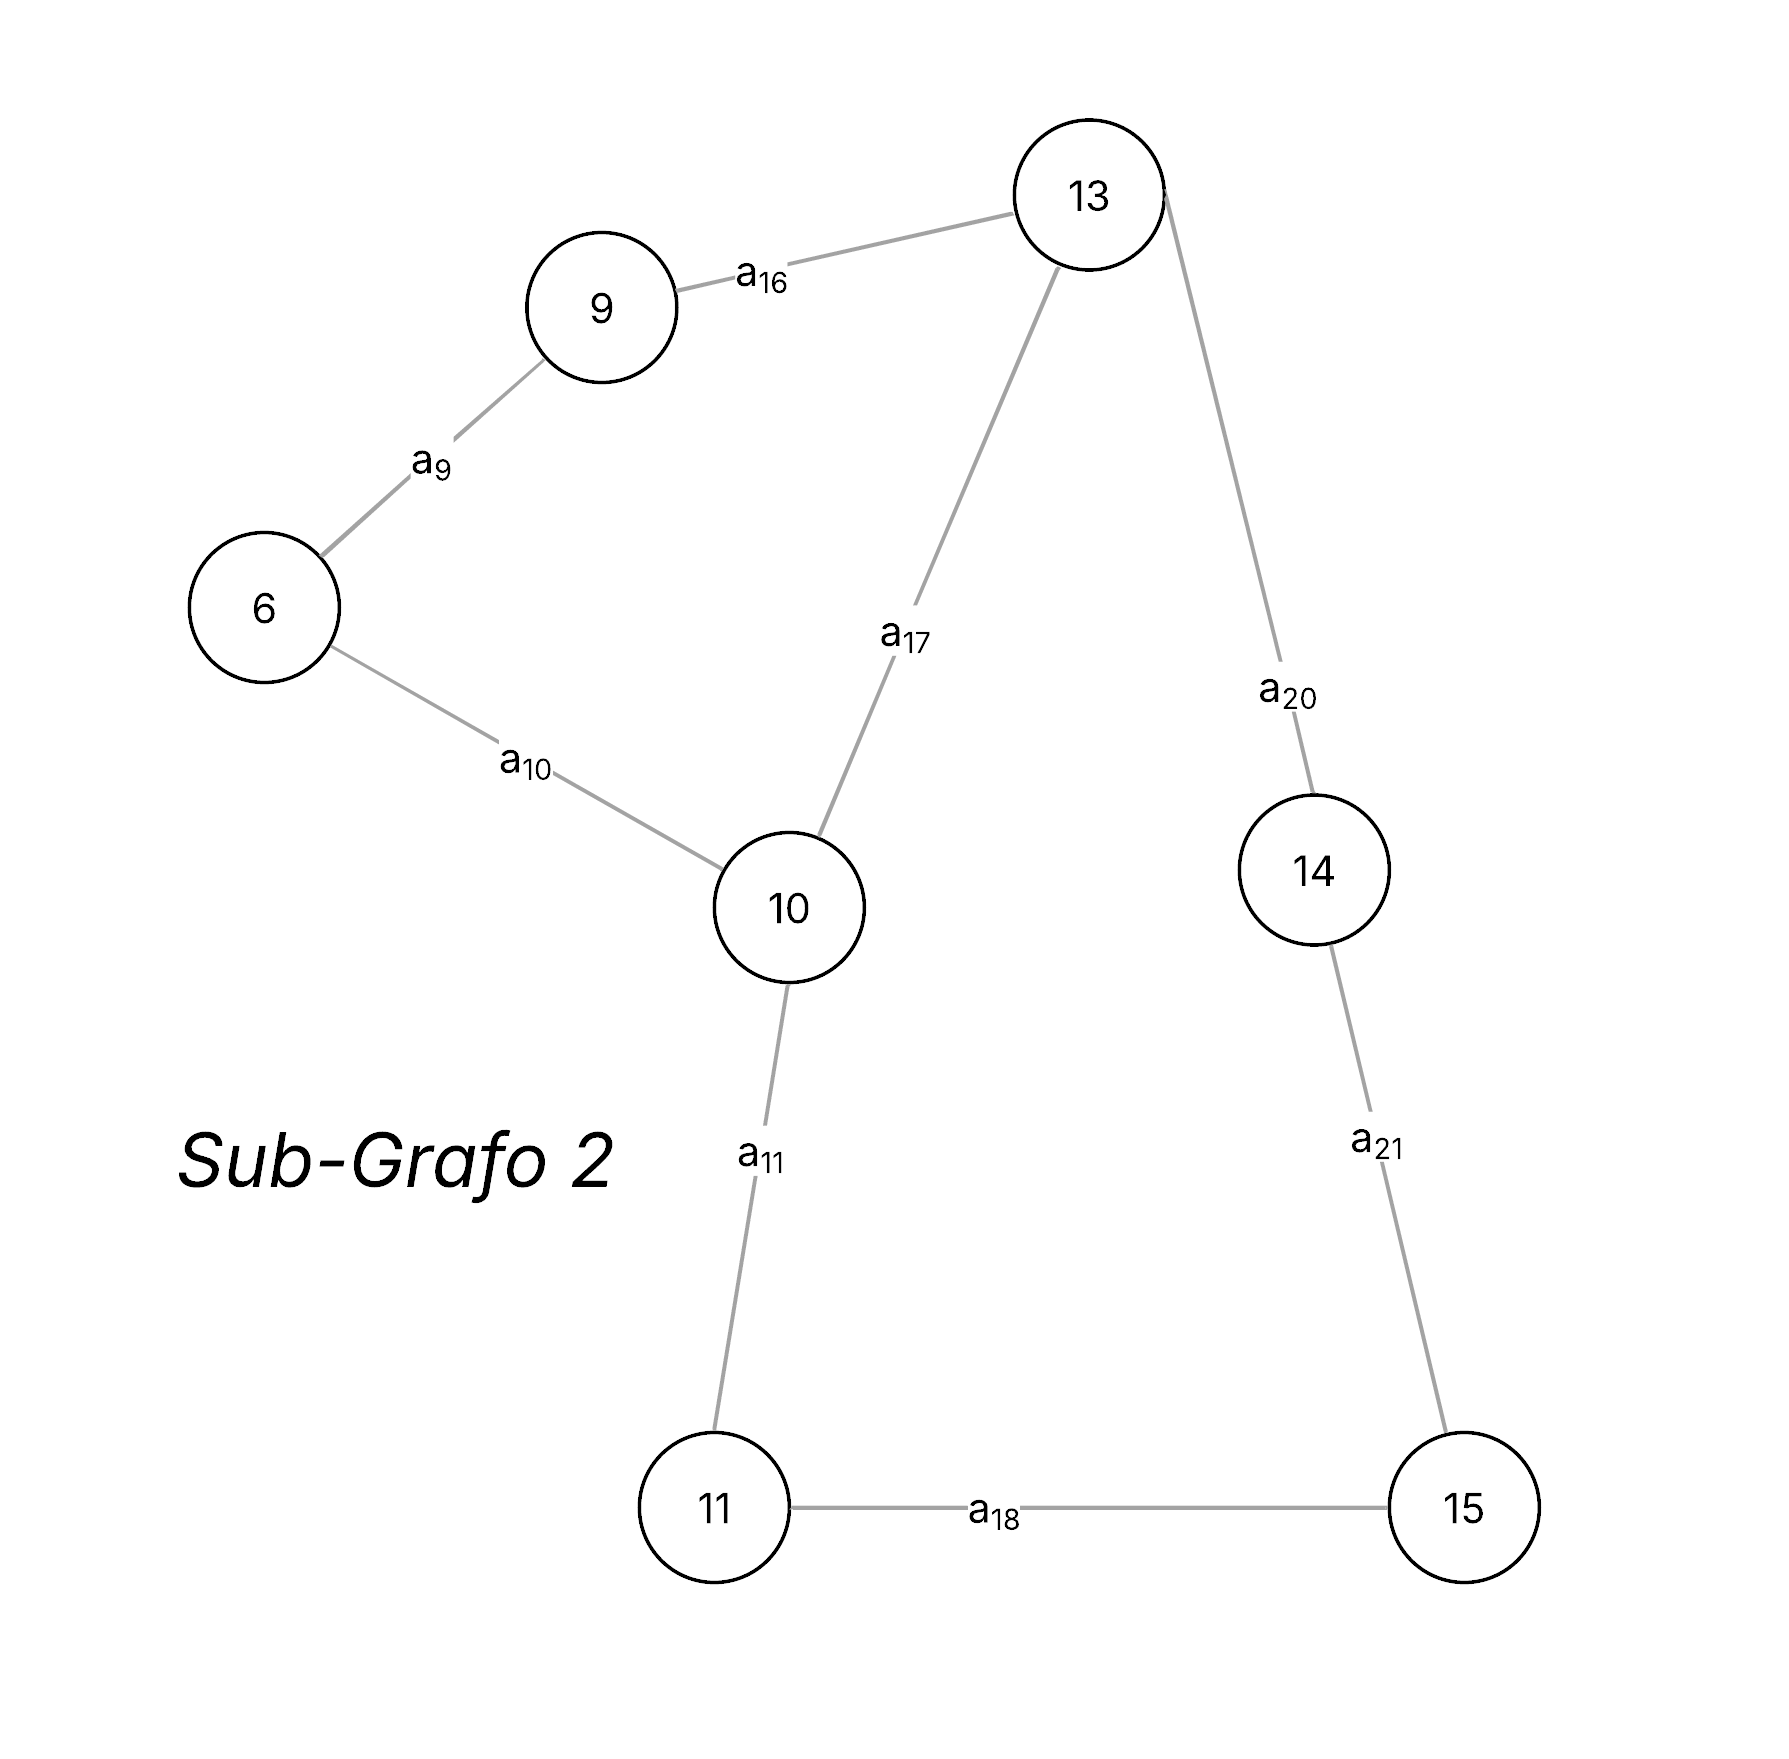
\includegraphics[width=\textwidth]{figuras/subgrafos/subgrafo2.png} % Substitua pelo caminho da sua imagem
                \caption{Sub-Grafo 2}
                \label{fig:imagem2}
            \end{subfigure}

            \caption{Sub-Grafos}
            \label{fig:duasFiguras}
        \end{figure}

    A aplicação da operação de união resultaria em $Sub\_Grafo1 \cup Sub\_Grafo2$, representando graficamente se dá na figura seguinte:

    \begin{figure}
        \centering
        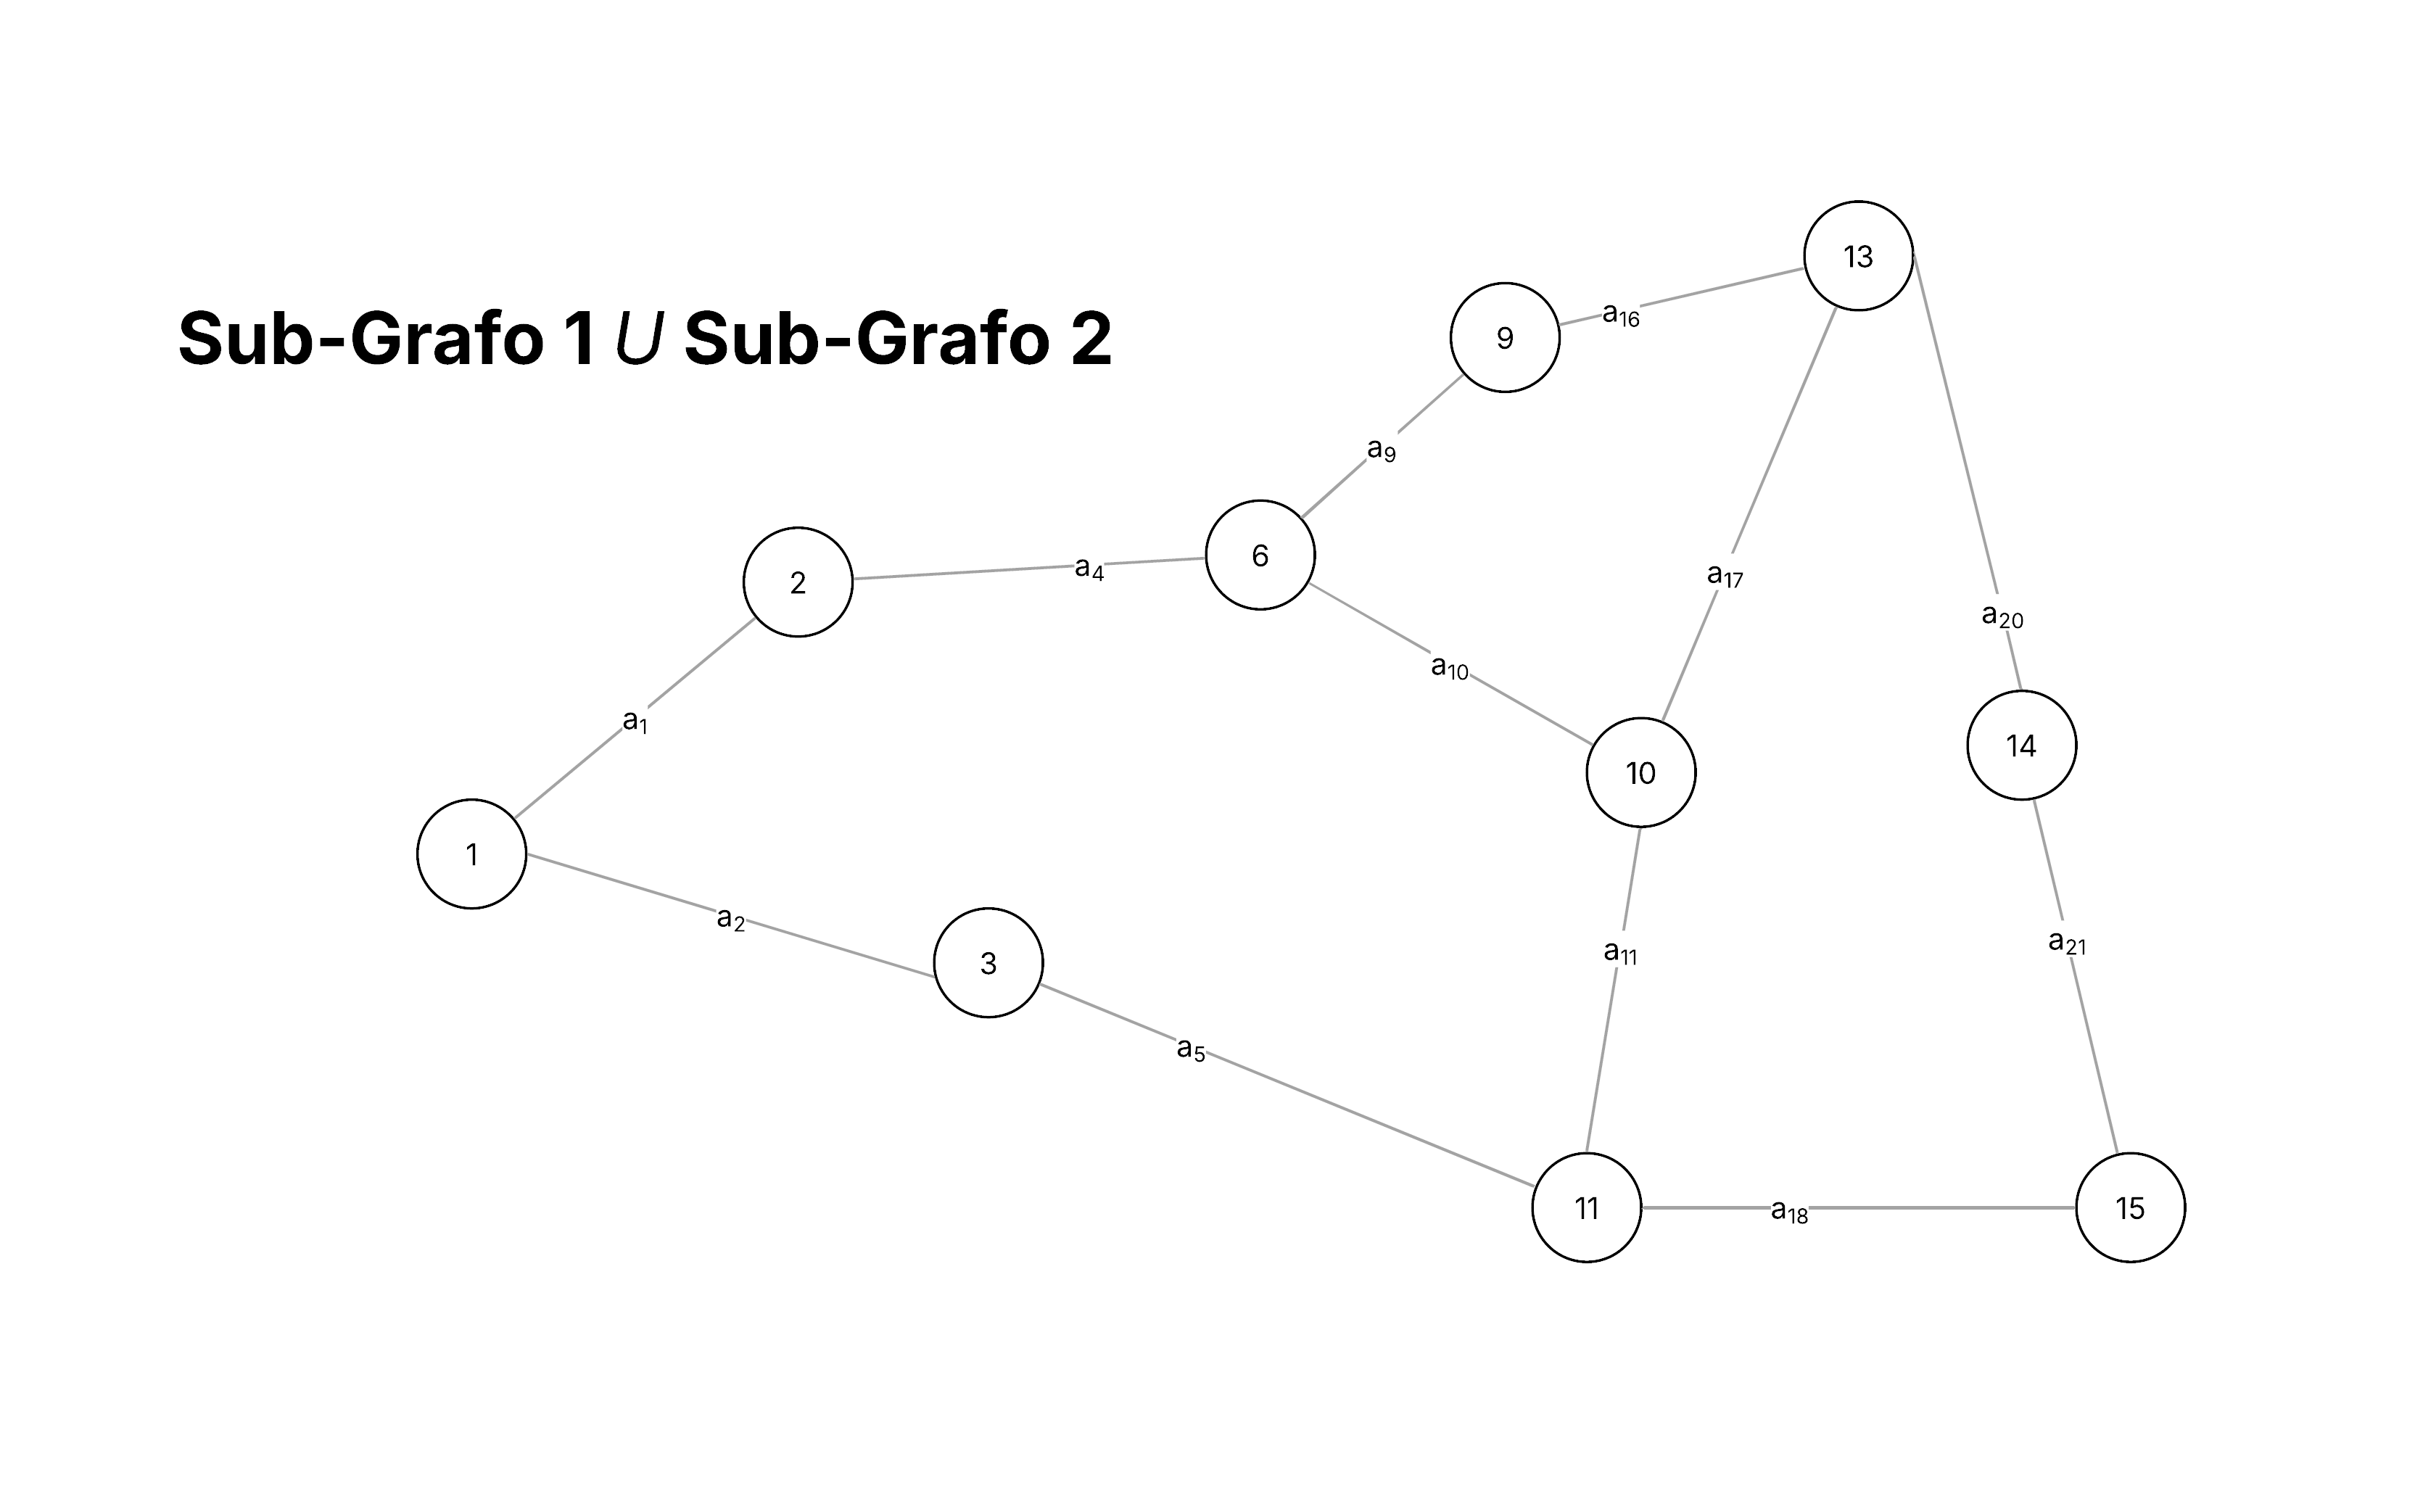
\includegraphics[width=0.8\textwidth]{figuras/subgrafos/subgrafo1usubgrafo2.png}
        \caption{União dos Sub-Grafos}
        \label{fig:uniaoGrafos}
    \end{figure}

	\section{Intersecção}\label{sec:interseccao}
	
	\section{Soma}\label{sec:soma}
	
	% Soma
	% Soma direta
	
	\section{Decomposição}\label{sec:decomposicao}
	
	\section{Remoção}\label{sec:remocao}
	
	% Remoção de uma aresta/arco
	% remoção de um vértice
	
	\section{Fusão de vértices}\label{sec:fusao}
	
	\section{Contração}\label{sec:contracao}
	% Contração de dois vértices
	% Contração de uma aresta
	
	
	\chapter{Buscas}\label{cap:buscas}
	
	A busca é umas das técnicas mais aplicadas na solução de problemas algorítmicos em grafos considerados eficientes. As duas técnicas de busca em grafos, a {dfs} e a {bfs}, são apresentadas, respectivamente, nas Seções \ref{sec:buscaLarg} e \ref{sec:buscaProf}.
	
	A Seção \ref{sec:compFC} apresenta uma aplicação das duas buscas para obter os componentes fortemente conexos de um grafo. As considerações acerca da eficiência computacional, tanto em relação ao tempo de processamento quanto ao espaço usado de memória pelas buscas, são dadas na Seção \ref{sec:eficienciaRepresentacao}.
	
	\section{Busca em Largura}\label{sec:buscaLarg}
	
	\section{Busca em Profundidade}\label{sec:buscaProf}
	
	\section{Componentes Fortemente Conexos}\label{sec:compFC}
	
	% Considerações de Eficiência
	\section{Considerações de Eficiência}\label{sec:eficienciaBusca}
	
	\chapter{CAMINHO MÍNIMO}\label{cap:caminhoMinimo}
	
	
	\chapter{ARVORE DE COBERTURA MÍNIMA}\label{cap:arvCobMinima}

	
	\chapter{GRAFOS EULERIANOS}\label{cap:grafosEulerianos}
	
	
	\chapter{GRAFOS HAMILTONIANOS}\label{cap:grafosHamiltonianos}
	
	
	\chapter{EMPARELHAMENTO}\label{cap:emparelhamento}

	
	\chapter{PLANARIDADE}\label{cap:planaridade}

	
	\chapter{COLORAÇÃO DE VÉRTICES}\label{cap:coloracaoVertices}

	
	% --- Referências (livre; substitua por biblatex se quiser)
	\clearpage
	\chapter*{REFERÊNCIAS}
	\addcontentsline{toc}{chapter}{REFERÊNCIAS}
	% Insira suas referências manualmente ou troque para biblatex.
	\vspace{-0.5em}
	\begin{itemize}
		\item \dots
	\end{itemize}
	
\end{document}
